\section{Potential Solution }
\label{sec:potentialsolution}
\begin{itemize}
	\item The biggest challenge I face, is the lack of knowledge in the field of medical procedures. I will be exploring the current technology being used for training and simulation in the health field in order to grasp the tasks and steps that will help with the creation of the studies using the Hololens. 
	\item Getting familiar with tools and devices being used is important, with no prior knowledge of medical procedures or analytical procedures to observe data, taking measures to understand the current state, as well as interviewing primary users such as medical professionals and scientists is crucial to developing effective guidelines for creating virtual information spaces for ARHWDs.
	\item I propose an algorithm that optimizes the placement of information based on certain criteria. This work aims to find that criteria as well as test the criteria against real-world applications and simulations. I will be looking at the efficiencies of different layouts while performing tasks, the way the windows adapt to visually busy areas, as well as what level of information about the should be displayed without confusing or impairing the task at hand.
\end{itemize}

\begin{figure}[h!]
  \centering
  \begin{subfigure}[b]{0.5\textwidth}
    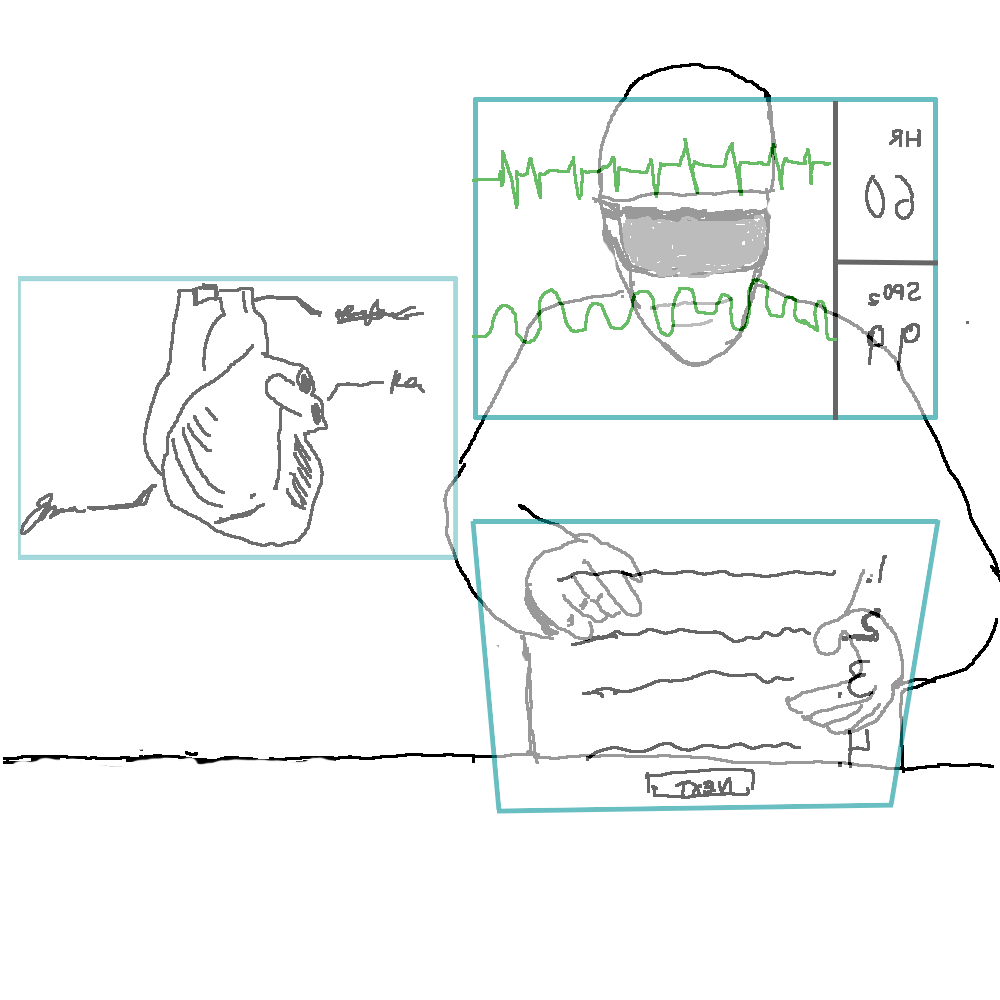
\includegraphics[width=\textwidth]{fig04.png}
    \caption{A sketch of the windows adapting to the head position with no busy areas.}
  \end{subfigure}
  \begin{subfigure}[b]{0.5\textwidth}
    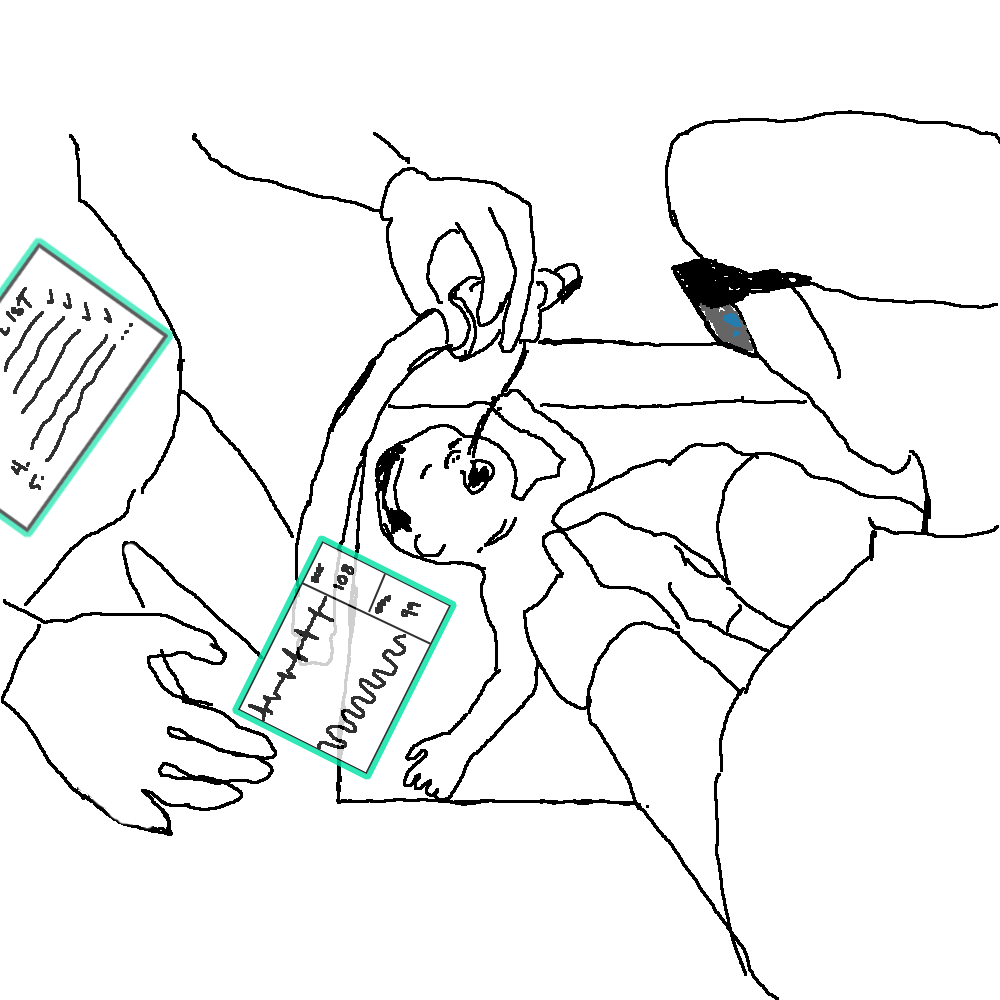
\includegraphics[width=\textwidth]{fig03.png}
    \caption{A sketch of the windows adapting to the head position in a busier area}
  \end{subfigure}
  \caption{Visually Flat Areas vs. Visually Busy Area}
  \label{fig:sketches}
\end{figure}
